\documentclass{standalone}
\usepackage{tikz}
\usetikzlibrary{patterns, positioning}


\begin{document}
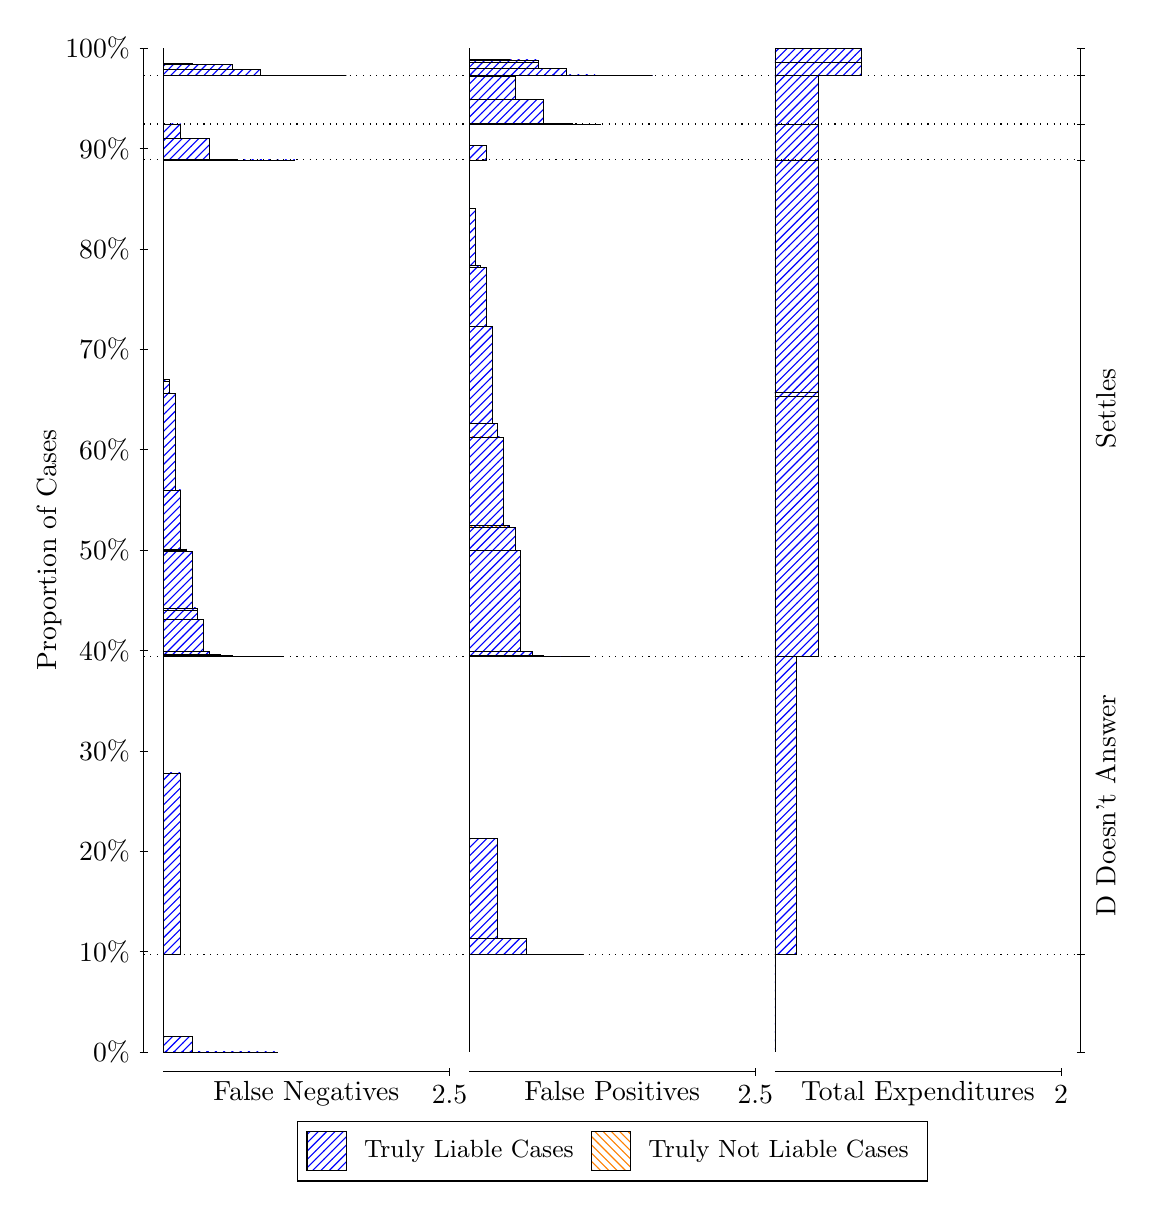
\begin{tikzpicture}
\draw[black, very thin] (1.5,1.75) -- (1.5,14.5);
\node[rotate=90, text=black, anchor=center] at (0.3, 8.125) {Proportion of Cases};
\draw[black, very thin] (1.45,1.75) -- (1.55,1.75);
\node[text=black, anchor=east] at (1.45, 1.75) {0\%};
\draw[black, very thin] (1.45,3.025) -- (1.55,3.025);
\node[text=black, anchor=east] at (1.45, 3.025) {10\%};
\draw[black, very thin] (1.45,4.3) -- (1.55,4.3);
\node[text=black, anchor=east] at (1.45, 4.3) {20\%};
\draw[black, very thin] (1.45,5.575) -- (1.55,5.575);
\node[text=black, anchor=east] at (1.45, 5.575) {30\%};
\draw[black, very thin] (1.45,6.85) -- (1.55,6.85);
\node[text=black, anchor=east] at (1.45, 6.85) {40\%};
\draw[black, very thin] (1.45,8.125) -- (1.55,8.125);
\node[text=black, anchor=east] at (1.45, 8.125) {50\%};
\draw[black, very thin] (1.45,9.4) -- (1.55,9.4);
\node[text=black, anchor=east] at (1.45, 9.4) {60\%};
\draw[black, very thin] (1.45,10.675) -- (1.55,10.675);
\node[text=black, anchor=east] at (1.45, 10.675) {70\%};
\draw[black, very thin] (1.45,11.95) -- (1.55,11.95);
\node[text=black, anchor=east] at (1.45, 11.95) {80\%};
\draw[black, very thin] (1.45,13.225) -- (1.55,13.225);
\node[text=black, anchor=east] at (1.45, 13.225) {90\%};
\draw[black, very thin] (1.45,14.5) -- (1.55,14.5);
\node[text=black, anchor=east] at (1.45, 14.5) {100\%};

\draw[black, very thin] (13.4,1.75) -- (13.4,14.5);
\draw[black, very thin] (13.35,1.75) -- (13.45,1.75);
\node[anchor=west] at (13.35, 1.75) {};
\draw[black, very thin] (13.35,2.9871) -- (13.45,2.9871);
\node[anchor=west] at (13.35, 2.9871) {};
\draw[black, very thin] (13.35,6.7731) -- (13.45,6.7731);
\node[anchor=west] at (13.35, 6.7731) {};
\draw[black, very thin] (13.35,13.079) -- (13.45,13.079);
\node[anchor=west] at (13.35, 13.079) {};
\draw[black, very thin] (13.35,13.535) -- (13.45,13.535);
\node[anchor=west] at (13.35, 13.535) {};
\draw[black, very thin] (13.35,14.151) -- (13.45,14.151);
\node[anchor=west] at (13.35, 14.151) {};
\draw[black, very thin] (13.35,14.5) -- (13.45,14.5);
\node[anchor=west] at (13.35, 14.5) {};

\draw[black, very thin, pattern color=blue, pattern=north east lines] (1.75,1.75) rectangle (3.2033,1.75);
\draw[black, very thin, pattern color=blue, pattern=north east lines] (1.75,1.75) rectangle (2.84,1.75);
\draw[black, very thin, pattern color=blue, pattern=north east lines] (1.75,1.75) rectangle (2.4767,1.7517);
\draw[black, very thin, pattern color=blue, pattern=north east lines] (1.75,1.7517) rectangle (2.1133,1.9526);
\draw[black, very thin, pattern color=orange, pattern=north west lines] (1.75,1.9526) rectangle (1.75,1.9526);
\draw[black, very thin, pattern color=blue, pattern=north east lines] (1.75,1.9526) rectangle (1.75,2.9871);
\draw[black, very thin, pattern color=blue, pattern=north east lines] (1.75,2.9871) rectangle (1.968,5.2946);
\draw[black, very thin, pattern color=orange, pattern=north west lines] (1.75,5.2946) rectangle (1.75,5.2946);
\draw[black, very thin, pattern color=blue, pattern=north east lines] (1.75,5.2946) rectangle (1.75,6.7731);
\draw[black, very thin, pattern color=blue, pattern=north east lines] (1.75,6.7731) rectangle (3.276,6.7731);
\draw[black, very thin, pattern color=blue, pattern=north east lines] (1.75,6.7731) rectangle (3.1307,6.7731);
\draw[black, very thin, pattern color=blue, pattern=north east lines] (1.75,6.7731) rectangle (2.9853,6.7731);
\draw[black, very thin, pattern color=blue, pattern=north east lines] (1.75,6.7731) rectangle (2.9127,6.7731);
\draw[black, very thin, pattern color=blue, pattern=north east lines] (1.75,6.7731) rectangle (2.84,6.7731);
\draw[black, very thin, pattern color=blue, pattern=north east lines] (1.75,6.7731) rectangle (2.7673,6.7731);
\draw[black, very thin, pattern color=blue, pattern=north east lines] (1.75,6.7731) rectangle (2.6947,6.7731);
\draw[black, very thin, pattern color=blue, pattern=north east lines] (1.75,6.7731) rectangle (2.622,6.7835);
\draw[black, very thin, pattern color=blue, pattern=north east lines] (1.75,6.7835) rectangle (2.5493,6.7845);
\draw[black, very thin, pattern color=blue, pattern=north east lines] (1.75,6.7845) rectangle (2.4767,6.8015);
\draw[black, very thin, pattern color=blue, pattern=north east lines] (1.75,6.8015) rectangle (2.404,6.8016);
\draw[black, very thin, pattern color=blue, pattern=north east lines] (1.75,6.8016) rectangle (2.404,6.8022);
\draw[black, very thin, pattern color=blue, pattern=north east lines] (1.75,6.8022) rectangle (2.3313,6.8351);
\draw[black, very thin, pattern color=blue, pattern=north east lines] (1.75,6.8351) rectangle (2.2587,7.2449);
\draw[black, very thin, pattern color=blue, pattern=north east lines] (1.75,7.2449) rectangle (2.186,7.3621);
\draw[black, very thin, pattern color=blue, pattern=north east lines] (1.75,7.3621) rectangle (2.186,7.3906);
\draw[black, very thin, pattern color=blue, pattern=north east lines] (1.75,7.3906) rectangle (2.1133,8.1103);
\draw[black, very thin, pattern color=blue, pattern=north east lines] (1.75,8.1103) rectangle (2.0407,8.1259);
\draw[black, very thin, pattern color=blue, pattern=north east lines] (1.75,8.1259) rectangle (2.0407,8.1382);
\draw[black, very thin, pattern color=blue, pattern=north east lines] (1.75,8.1382) rectangle (1.968,8.8885);
\draw[black, very thin, pattern color=blue, pattern=north east lines] (1.75,8.8885) rectangle (1.8953,10.121);
\draw[black, very thin, pattern color=blue, pattern=north east lines] (1.75,10.121) rectangle (1.8227,10.269);
\draw[black, very thin, pattern color=blue, pattern=north east lines] (1.75,10.269) rectangle (1.8227,10.291);
\draw[black, very thin, pattern color=orange, pattern=north west lines] (1.75,10.291) rectangle (1.75,10.291);
\draw[black, very thin, pattern color=blue, pattern=north east lines] (1.75,10.291) rectangle (1.75,13.079);
\draw[black, very thin, pattern color=blue, pattern=north east lines] (1.75,13.079) rectangle (3.4213,13.079);
\draw[black, very thin, pattern color=blue, pattern=north east lines] (1.75,13.079) rectangle (3.058,13.079);
\draw[black, very thin, pattern color=blue, pattern=north east lines] (1.75,13.079) rectangle (2.6947,13.086);
\draw[black, very thin, pattern color=blue, pattern=north east lines] (1.75,13.086) rectangle (2.3313,13.352);
\draw[black, very thin, pattern color=blue, pattern=north east lines] (1.75,13.352) rectangle (1.968,13.535);
\draw[black, very thin, pattern color=orange, pattern=north west lines] (1.75,13.535) rectangle (1.75,13.535);
\draw[black, very thin, pattern color=blue, pattern=north east lines] (1.75,13.535) rectangle (1.968,13.538);
\draw[black, very thin, pattern color=orange, pattern=north west lines] (1.75,13.538) rectangle (1.75,13.538);
\draw[black, very thin, pattern color=blue, pattern=north east lines] (1.75,13.538) rectangle (1.75,14.151);
\draw[black, very thin, pattern color=blue, pattern=north east lines] (1.75,14.151) rectangle (4.0753,14.151);
\draw[black, very thin, pattern color=blue, pattern=north east lines] (1.75,14.151) rectangle (3.712,14.151);
\draw[black, very thin, pattern color=blue, pattern=north east lines] (1.75,14.151) rectangle (3.3487,14.156);
\draw[black, very thin, pattern color=blue, pattern=north east lines] (1.75,14.156) rectangle (2.9853,14.228);
\draw[black, very thin, pattern color=blue, pattern=north east lines] (1.75,14.228) rectangle (2.84,14.228);
\draw[black, very thin, pattern color=blue, pattern=north east lines] (1.75,14.228) rectangle (2.622,14.291);
\draw[black, very thin, pattern color=blue, pattern=north east lines] (1.75,14.291) rectangle (2.4767,14.291);
\draw[black, very thin, pattern color=blue, pattern=north east lines] (1.75,14.291) rectangle (2.2587,14.292);
\draw[black, very thin, pattern color=blue, pattern=north east lines] (1.75,14.292) rectangle (2.1133,14.3);
\draw[black, very thin, pattern color=blue, pattern=north east lines] (1.75,14.3) rectangle (1.8953,14.3);
\draw[black, very thin, pattern color=orange, pattern=north west lines] (1.75,14.3) rectangle (1.75,14.3);
\draw[black, very thin, pattern color=blue, pattern=north east lines] (1.75,14.3) rectangle (1.75,14.5);
\draw[black, very thin, pattern color=orange, pattern=north west lines] (5.6333,1.75) rectangle (5.6333,1.75);
\draw[black, very thin, pattern color=blue, pattern=north east lines] (5.6333,1.75) rectangle (5.6333,2.9871);
\draw[black, very thin, pattern color=orange, pattern=north west lines] (5.6333,2.9871) rectangle (7.0867,2.9871);
\draw[black, very thin, pattern color=blue, pattern=north east lines] (5.6333,2.9871) rectangle (7.0867,2.9871);
\draw[black, very thin, pattern color=blue, pattern=north east lines] (5.6333,2.9871) rectangle (6.7233,2.9886);
\draw[black, very thin, pattern color=blue, pattern=north east lines] (5.6333,2.9886) rectangle (6.36,3.1923);
\draw[black, very thin, pattern color=blue, pattern=north east lines] (5.6333,3.1923) rectangle (5.9967,4.4656);
\draw[black, very thin, pattern color=blue, pattern=north east lines] (5.6333,4.4656) rectangle (5.6333,6.7731);
\draw[black, very thin, pattern color=orange, pattern=north west lines] (5.6333,6.7731) rectangle (7.1593,6.7731);
\draw[black, very thin, pattern color=blue, pattern=north east lines] (5.6333,6.7731) rectangle (7.1593,6.7731);
\draw[black, very thin, pattern color=orange, pattern=north west lines] (5.6333,6.7731) rectangle (6.8687,6.7731);
\draw[black, very thin, pattern color=blue, pattern=north east lines] (5.6333,6.7731) rectangle (6.8687,6.7731);
\draw[black, very thin, pattern color=blue, pattern=north east lines] (5.6333,6.7731) rectangle (6.796,6.7731);
\draw[black, very thin, pattern color=orange, pattern=north west lines] (5.6333,6.7731) rectangle (6.7233,6.7731);
\draw[black, very thin, pattern color=blue, pattern=north east lines] (5.6333,6.7731) rectangle (6.7233,6.7731);
\draw[black, very thin, pattern color=orange, pattern=north west lines] (5.6333,6.7731) rectangle (6.578,6.7731);
\draw[black, very thin, pattern color=blue, pattern=north east lines] (5.6333,6.7731) rectangle (6.578,6.7835);
\draw[black, very thin, pattern color=blue, pattern=north east lines] (5.6333,6.7835) rectangle (6.5053,6.7836);
\draw[black, very thin, pattern color=orange, pattern=north west lines] (5.6333,6.7836) rectangle (6.4327,6.7836);
\draw[black, very thin, pattern color=blue, pattern=north east lines] (5.6333,6.7836) rectangle (6.4327,6.8369);
\draw[black, very thin, pattern color=blue, pattern=north east lines] (5.6333,6.8369) rectangle (6.36,6.8386);
\draw[black, very thin, pattern color=orange, pattern=north west lines] (5.6333,6.8386) rectangle (6.2873,6.8386);
\draw[black, very thin, pattern color=blue, pattern=north east lines] (5.6333,6.8386) rectangle (6.2873,8.1195);
\draw[black, very thin, pattern color=blue, pattern=north east lines] (5.6333,8.1195) rectangle (6.2147,8.4182);
\draw[black, very thin, pattern color=orange, pattern=north west lines] (5.6333,8.4182) rectangle (6.142,8.4182);
\draw[black, very thin, pattern color=blue, pattern=north east lines] (5.6333,8.4182) rectangle (6.142,8.4347);
\draw[black, very thin, pattern color=blue, pattern=north east lines] (5.6333,8.4347) rectangle (6.0693,9.5602);
\draw[black, very thin, pattern color=orange, pattern=north west lines] (5.6333,9.5602) rectangle (5.9967,9.5602);
\draw[black, very thin, pattern color=blue, pattern=north east lines] (5.6333,9.5602) rectangle (5.9967,9.7304);
\draw[black, very thin, pattern color=blue, pattern=north east lines] (5.6333,9.7304) rectangle (5.924,10.963);
\draw[black, very thin, pattern color=blue, pattern=north east lines] (5.6333,10.963) rectangle (5.8513,11.713);
\draw[black, very thin, pattern color=blue, pattern=north east lines] (5.6333,11.713) rectangle (5.7787,11.741);
\draw[black, very thin, pattern color=blue, pattern=north east lines] (5.6333,11.741) rectangle (5.706,12.461);
\draw[black, very thin, pattern color=blue, pattern=north east lines] (5.6333,12.461) rectangle (5.6333,13.079);
\draw[black, very thin, pattern color=orange, pattern=north west lines] (5.6333,13.079) rectangle (5.8513,13.079);
\draw[black, very thin, pattern color=blue, pattern=north east lines] (5.6333,13.079) rectangle (5.8513,13.261);
\draw[black, very thin, pattern color=blue, pattern=north east lines] (5.6333,13.261) rectangle (5.6333,13.535);
\draw[black, very thin, pattern color=orange, pattern=north west lines] (5.6333,13.535) rectangle (7.3047,13.535);
\draw[black, very thin, pattern color=blue, pattern=north east lines] (5.6333,13.535) rectangle (7.3047,13.535);
\draw[black, very thin, pattern color=blue, pattern=north east lines] (5.6333,13.535) rectangle (6.9413,13.539);
\draw[black, very thin, pattern color=blue, pattern=north east lines] (5.6333,13.539) rectangle (6.578,13.848);
\draw[black, very thin, pattern color=blue, pattern=north east lines] (5.6333,13.848) rectangle (6.2147,14.147);
\draw[black, very thin, pattern color=blue, pattern=north east lines] (5.6333,14.147) rectangle (5.8513,14.151);
\draw[black, very thin, pattern color=orange, pattern=north west lines] (5.6333,14.151) rectangle (7.9587,14.151);
\draw[black, very thin, pattern color=blue, pattern=north east lines] (5.6333,14.151) rectangle (7.9587,14.151);
\draw[black, very thin, pattern color=orange, pattern=north west lines] (5.6333,14.151) rectangle (7.5953,14.151);
\draw[black, very thin, pattern color=blue, pattern=north east lines] (5.6333,14.151) rectangle (7.5953,14.151);
\draw[black, very thin, pattern color=orange, pattern=north west lines] (5.6333,14.151) rectangle (7.232,14.151);
\draw[black, very thin, pattern color=blue, pattern=north east lines] (5.6333,14.151) rectangle (7.232,14.158);
\draw[black, very thin, pattern color=blue, pattern=north east lines] (5.6333,14.158) rectangle (6.8687,14.237);
\draw[black, very thin, pattern color=orange, pattern=north west lines] (5.6333,14.237) rectangle (6.8687,14.237);
\draw[black, very thin, pattern color=blue, pattern=north east lines] (5.6333,14.237) rectangle (6.8687,14.238);
\draw[black, very thin, pattern color=blue, pattern=north east lines] (5.6333,14.238) rectangle (6.5053,14.32);
\draw[black, very thin, pattern color=blue, pattern=north east lines] (5.6333,14.32) rectangle (6.5053,14.35);
\draw[black, very thin, pattern color=orange, pattern=north west lines] (5.6333,14.35) rectangle (6.36,14.35);
\draw[black, very thin, pattern color=blue, pattern=north east lines] (5.6333,14.35) rectangle (6.36,14.35);
\draw[black, very thin, pattern color=blue, pattern=north east lines] (5.6333,14.35) rectangle (6.142,14.351);
\draw[black, very thin, pattern color=blue, pattern=north east lines] (5.6333,14.351) rectangle (6.142,14.359);
\draw[black, very thin, pattern color=orange, pattern=north west lines] (5.6333,14.359) rectangle (5.9967,14.359);
\draw[black, very thin, pattern color=blue, pattern=north east lines] (5.6333,14.359) rectangle (5.9967,14.36);
\draw[black, very thin, pattern color=blue, pattern=north east lines] (5.6333,14.36) rectangle (5.7787,14.36);
\draw[black, very thin, pattern color=blue, pattern=north east lines] (5.6333,14.36) rectangle (5.7787,14.36);
\draw[black, very thin, pattern color=orange, pattern=north west lines] (5.6333,14.36) rectangle (5.6333,14.36);
\draw[black, very thin, pattern color=blue, pattern=north east lines] (5.6333,14.36) rectangle (5.6333,14.5);
\draw[black, very thin, pattern color=orange, pattern=north west lines] (9.5167,1.75) rectangle (9.5167,1.75);
\draw[black, very thin, pattern color=blue, pattern=north east lines] (9.5167,1.75) rectangle (9.5167,2.9871);
\draw[black, very thin, pattern color=orange, pattern=north west lines] (9.5167,2.9871) rectangle (9.7892,2.9871);
\draw[black, very thin, pattern color=blue, pattern=north east lines] (9.5167,2.9871) rectangle (9.7892,6.7731);
\draw[black, very thin, pattern color=orange, pattern=north west lines] (9.5167,6.7731) rectangle (10.062,6.7731);
\draw[black, very thin, pattern color=blue, pattern=north east lines] (9.5167,6.7731) rectangle (10.062,10.079);
\draw[black, very thin, pattern color=orange, pattern=north west lines] (9.5167,10.079) rectangle (10.062,10.079);
\draw[black, very thin, pattern color=blue, pattern=north east lines] (9.5167,10.079) rectangle (10.062,10.131);
\draw[black, very thin, pattern color=orange, pattern=north west lines] (9.5167,10.131) rectangle (10.062,10.131);
\draw[black, very thin, pattern color=blue, pattern=north east lines] (9.5167,10.131) rectangle (10.062,13.079);
\draw[black, very thin, pattern color=orange, pattern=north west lines] (9.5167,13.079) rectangle (10.062,13.079);
\draw[black, very thin, pattern color=blue, pattern=north east lines] (9.5167,13.079) rectangle (10.062,13.535);
\draw[black, very thin, pattern color=orange, pattern=north west lines] (9.5167,13.535) rectangle (10.062,13.535);
\draw[black, very thin, pattern color=blue, pattern=north east lines] (9.5167,13.535) rectangle (10.062,14.151);
\draw[black, very thin, pattern color=orange, pattern=north west lines] (9.5167,14.151) rectangle (10.607,14.151);
\draw[black, very thin, pattern color=blue, pattern=north east lines] (9.5167,14.151) rectangle (10.607,14.321);
\draw[black, very thin, pattern color=orange, pattern=north west lines] (9.5167,14.321) rectangle (10.607,14.321);
\draw[black, very thin, pattern color=blue, pattern=north east lines] (9.5167,14.321) rectangle (10.607,14.5);
\draw[black, dotted] (1.5,2.9871) -- (13.4,2.9871);
\draw[black, dotted] (1.5,6.7731) -- (13.4,6.7731);
\draw[black, dotted] (1.5,13.079) -- (13.4,13.079);
\draw[black, dotted] (1.5,13.535) -- (13.4,13.535);
\draw[black, dotted] (1.5,14.151) -- (13.4,14.151);
\draw[black, very thin] (1.75,1.5) -- (5.3833,1.5);
\node[text=black, anchor=north] at (3.5667, 1.5) {False Negatives};
\draw[black, very thin] (5.3833,1.45) -- (5.3833,1.55);
\node[text=black, anchor=north] at (5.3833, 1.45) {2.5};

\draw[black, very thin] (5.6333,1.5) -- (9.2667,1.5);
\node[text=black, anchor=north] at (7.45, 1.5) {False Positives};
\draw[black, very thin] (9.2667,1.45) -- (9.2667,1.55);
\node[text=black, anchor=north] at (9.2667, 1.45) {2.5};

\draw[black, very thin] (9.5167,1.5) -- (13.15,1.5);
\node[text=black, anchor=north] at (11.333, 1.5) {Total Expenditures};
\draw[black, very thin] (13.15,1.45) -- (13.15,1.55);
\node[text=black, anchor=north] at (13.15, 1.45) {2};


\node[text=black, centered, rotate=90] at (13.72, 4.8801) {D Doesn't Answer};
\node[text=black, centered, rotate=90] at (13.72, 9.9258) {Settles};




\draw (7.449999999999999,1.5) node[draw=none] (baseCoordinate) {};
\begin{scope}[align=center]
        \matrix[scale=0.5, draw=black, below=0.5cm of baseCoordinate, nodes={draw}, column sep=0.1cm]{
            \node[rectangle, draw, minimum width=0.5cm, minimum height=0.5cm, pattern color=blue, pattern=north east lines] {}; &
            \node[draw=none, font=\small, text=black] (B) {Truly Liable Cases}; &
            \node[rectangle, draw, minimum width=0.5cm, minimum height=0.5cm, pattern color=orange, pattern=north west lines] {}; &
            \node[draw=none, font=\small, text=black] (B) {Truly Not Liable Cases}; \\
            };
\end{scope}

\end{tikzpicture}
\end{document}